\section{Méthode}

\subsection{Dataset}

Nous utilisons le dataset fournit pour la tâche 3 de l’édition 2009 de DEFT.
Au moment de faire des statistiques descriptives, nous nous sommes rendu compte 
que le corpus présentait de nombreux doublons.
\begin{figure}[ht]
    \centering
    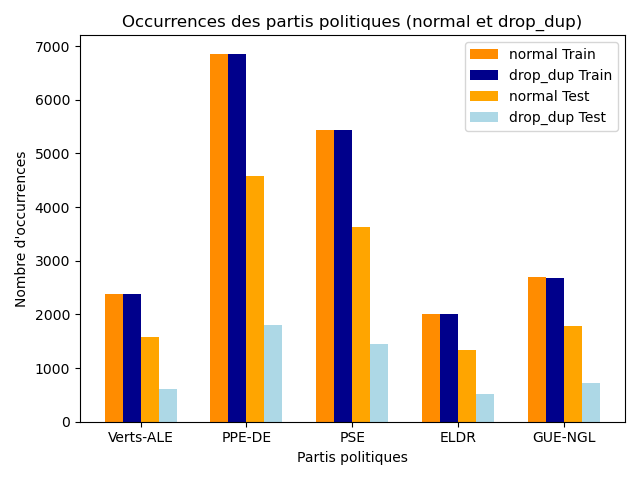
\includegraphics[width=\columnwidth]{../stats/occurences_orig_vs_drop_dup_par_cat.png}
    \caption{Nombre d'interventions par parti par partition test/train, dans le corpus original et dans la version sans doublons}
    \label{fig:barplot_dataset}
\end{figure}

Après suppression des doublons, la partition prévue n'est plus respectée : elle est 
passée de 40/60 à 20/80\footnote{ 0.79 pour le train et 0.21 pour le test}.
Nous avons envisagé de rétablir le partitionnement prévu, mais avons renoncé pour deux raisons. Tout d'abord,  
refaire le partitionnement nous aurait éloigné encore plus du corpus initial. De plus, des expériences préliminaires sur quelques modèles
n'ont montré que peu de changement avec les résultats de la partition 20/80.\\
Par ailleurs, la répartition des classes est déséquilibrée : les classes PPE-DE et PSE sont plus fournies et forment à elles deux 63,5 \% du corpus. Ceci sera
pris en compte dans les prétraitements.\footnote{la figure correspond au train, mais la répartition est sensiblement la même dans le test}

\begin{table}[ht]
    \centering
\begin{tabular}{|l|l|l|}
\hline
Statistique & Train & Test \\ \hline
Moyenne & 3871.4 & 1021.2 \\ \hline
STD & 2149.1 & 569.7 \\ \hline
Min & 2005.0 & 525.0 \\ \hline
1er quartile & 2376.0 & 615.0 \\ \hline
Médiane & 2687.0 & 715.0\\ \hline
3eme quartile & 5431.0 & 1448.0\\ \hline
Max & 6858.0 & 1803.0\\ \hline
\end{tabular}
\caption{Nombre d'interventions des partis par partition}
\label{tab:stats_dataset}
\end{table}

\begin{figure}[ht]
    \centering
    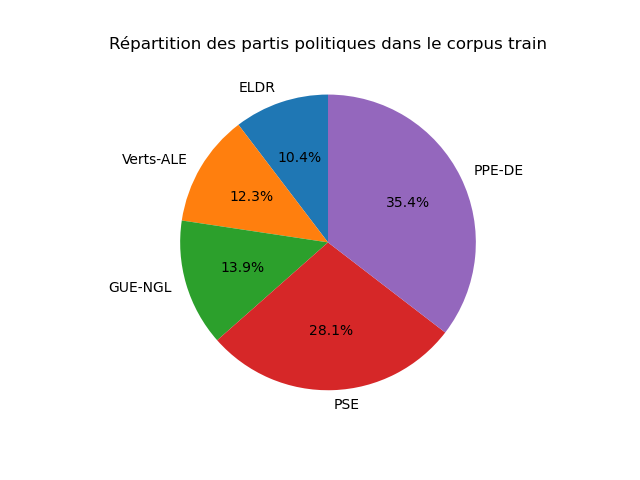
\includegraphics[width=\columnwidth]{../stats/occurences_par_partis_train_camember.png}
    \caption{Répartition des interventions par parti dans la partition train sans doublons}
    \label{fig:camember_dataset}
\end{figure}
\subsection{Prétraitements}
Le texte des interventions a été soumis à un prétraitement simple :\\
\indent(1) Suppression de la ponctuation\\
\indent(2) Unification de la casse en minuscules\\
\indent(3) Tokenisation\footnote {Une lemmatisation avec la bibliothèque \texttt{SpaCy} a été envisagée,
mais ce corpus multilingue aurait nécessité le chargement de 3 modèles linguistiques
différents et ralongé d'autant le temps de traitement}
\\
Pour résoudre le problème du déséquilibre des classes, nous avons opté pour le 
\textit{downsampling} en utilisant la fonction \textit{resample} de la bibliothèque \texttt{sckit-learn}. Nous avons choisi de downsampler les deux classes majoritaires en fonction de la médiane du nombre de documents sur toutes les classes. Après \textit{downsampling},
les classes PPE-DE et PSE ne représentent plus que 43\% du corpus, ayant chacune été ramenée autour de 21,5\% du corpus.

\begin{table}[ht]
    \centering
\begin{tabular}{|l|l|l|}
\hline
Parti & Train & Test\\ \hline
ELDR & 2531 (16,1\%) & 525 (16,2\%) \\ \hline
PPE-DE & 3402 (21,63\%) & 715 (22\%) \\ \hline
GUE-NGL & 3402 (21,63\%) & 687 (21,2\%) \\ \hline
PSE & 3402 (21,63\%) & 693 (21,4\%) \\ \hline
Verts-ALE & 2990 (19\%) & 614 (19\%)\\ \hline
Total & 15727 & 3235\\ \hline
\end{tabular}
\caption{Nombre d'interventions par parti par partition pour une langue après \textit{downsampling}, example de l'italien}
\label{tab:stats_downsampled}
\end{table}

\subsection{Les différents classifieurs testés}

Nous avons sélectionné quatre modèles classiques de machine learning, à savoir Random Forest, Support Vector Machine (SVM),  Régression Logistique et Perceptron.

\par Le \textbf{Random Forest} est une forêt d'arbres de décision qui utilise le \textit{bagging} pour améliorer la qualité des prédictions. L'algorithme fonctionne par une combinaison des résultats de multiples arbres construits sur des sous-échantillons pris aléatoirement dans le corpus.

\par Le \textbf{SVM}, quant à lui, repose sur l'idée de trouver un hyperplan optimal pour séparer les classes qui garantit une marge maximale. L'algorithme utilise une fonction noyau pour transformer les données et ajouter un espace de dimension supplémentaire, ce qui permet de résoudre des problèmes de classification non linéaire tout en utilisant tout de même un classifieur linéaire.

\par La \textbf{Régression Logistique} modélise la probabilité qu'un échantillon appartienne à une classe en utilisant une fonction sigmoïde. Elle nécessite une relation linéaire entre les \textit{features} et la classe.

\par Enfin, le \textbf{Perceptron} est un modèle de réseau de neurones linéaire qui ajuste les poids d'un seul neurone en fonction de l'erreur de prédiction, optimisé via une descente de gradient.

\par Ces quatre modèles ont été selectionnés car complémentaires : ils permettent d'aborder le problème sous différentes angles, avec des approches plus adaptées à la linéarité et d'autres à la non linéarité.



\subsection{Les différents vecteurs testés}
Nous avons choisi dans notre étude de comparer les résultats obtenus sur une tâche 
de classification en utilisant 3 techniques de vectorisation différentes.\\
\indent La vectorisation \textbf{\texttt{TF-IDF}}\footnote{Implémentée avec la fonction \texttt{tfidfvectorizer} de \texttt{scikit-learn}}(\textit{Term Frequency-Inverse Document Frequency})
est la seule méthode non neuronale que nous présentons, en ce qu'elle se fonde sur des statistiques. La fréquence d'apparition de chaque mot dans un document est divisée par sa fréquence d'apparition dans le corpus,
permettant de donner plus d'importance aux mots significatifs dans leurs documents d'apparition.\\
\indent La vectorisation \textbf{\texttt{Doc2Vec}}\footnote{Implémentée à l'aide de la bibliothèque \texttt{gensim}} génère un \textit{embedding} pour chaque document. Ces vecteurs sont
\textit{l'ouput} d'un réseau de neurones à mémoire distribuée. Pour cette étude,
nous avons choisi de générer des vecteurs \texttt{Doc2Vec} à 100 dimensions\footnote{Bien que des dimensions plus élevées puissent améliorer la capacité de représentation, nous avons choisi cette configuration pour ne pas saturer nos ressources matérielles.}
avec une fenêtre glissante de 5 mots et d'ignorer les mots n'apparaissant pas au moins 3 fois.\\
\indent La vectorisation avec \textbf{\texttt{BERT}} multilingue\footnote{\textit{bert-base-multilingual-uncased}} se base sur les réseaux de neurones mais s'appuie sur une 
architecture transformer caractérisée par ses mécanismes d'attention. Contrairement à
\texttt{Doc2Vec}, \texttt{BERT} produit des \textit{embeddings} au niveau des tokens, qui peuvent être agrégés pour obtenir un vecteur document. Nous avons généré des vecteurs à 768 dimensions (profondeur de la couche de sortie finale du modèle pré-entrainé).





